
\documentclass[11pt]{article}
\usepackage{hyperref}
\usepackage{mathtools}
\usepackage{pgfplots}
\begin{document}
    \section*{\huge \centering Matematica Discreta e Probabilit\'a }
     \subsection*{Suddivisione corso} 
        Il corso \`e suddiviso in quattro parti: calcolo combinatorio,
        statistica descrittiva, probabilit\'a e statistica inferenziale. \\
        Verranno dedicate 10 ore per la parte di calcolo combinatorio, 5 
        per la parte di statistica descrittiva, 40 per la parte di probabilit\'a e 5 per la parte di statistica inferenziale.
   \section{Calcolo Combinatorio}
    \subsection{Richiami}
        Serviranno i concetti di \textbf{insieme},\textbf{ sottoinsieme}, e di funzioni \textbf{iniettive} e \textbf{suriettive}.
        \subsubsection{Insieme}
            Un \textbf{insieme} \`e un raggruppamento di elementi che pu\'o essere individuato mediante una caratteristica comune che gli appartengono.\\
            $A=\{a,b\}$
        \subsubsection{Sottoinsieme}
            Un \textbf{sottoinsieme} \`e un raggruppamento di elementi appartenenti ad un insieme che \`e anch'esso un insieme.\\
            $B=\{n \in N : 1\leq n \leq 5 \} $ 
        \subsubsection{Funzioni Iniettive}
            Una funzione si dice \textbf{Iniettiva} se elementi distinti del dominio hanno immagini distinte. Possono esistere elementi del codominio non raggiunto da elementi del dominio.
        \subsubsection{Funzioni Suriettive}
            Una funzione si dice \textbf{Suriettiva} se ogni elemento del codominio \`e raggiunto da almeno un elemento del dominio. Non possono esistere elementi del codominio non raggiunto da elementi del dominio.
        \subsubsection{Funzioni Biettive}
            Una funzione si dice \textbf{Biettiva} se \`e sia suriettiva che iniettiva.
    \subsection{Teoria della Cardinalit\'a}
        Due insiemi hanno la stessa \textbf{cardinalit\'a} se esiste una biezione tra essi.\\
        Se \`e possibile costruire una funzione biettiva tra due insiemi.
        \subsubsection{Definizioni}
            Un insieme $A$ si dice finito se esiste $n \geq 0$ tale che $A$ e $\{1,2,..n\}$ hanno la stessa \textbf{cardinalit\'a}.  \\
            \\
            Se $A \longleftrightarrow \{1,..,n\}$ diciamo che $A$ ha \textbf{cardinalit\'a} $n$ e scriviamo  
            $|A|  =  n $ 
            \\
            \\
            Un insieme $A$ si dice \textbf{numerabile} se esiste biezione. 
            $A \longleftrightarrow N = \{0,1,2,..\}$
        \subsubsection{Esempi}
            \textbf{\large 1}\\
            $B=\{1,2,3,..\} \ \ f:N\to B , f(n)=n+1 $ \\
            La funzione rappresenta la corrispondenza tra $B$ e l'insieme dei numeri interi positivi (infiniti) $\mapsto$ $B$ \`e \textbf{numerabile}.\\
            \textbf{\large 2}\\
            $Z=\{0,1,-1,2,-2,..\}$ \`e \textbf{numerabile}? \\
            Si, lo \`e perch\`e basta fare le giuste associazioni : \\
            $0\mapsto 0 $, $1\mapsto1$, $-1\mapsto2$, $2\mapsto3$\\
            $f:Z\to N$ $\{2z-1 $ se $z>0$ \\
            \hspace*{1,8cm} $\{-2z  $ \hspace{0,35cm}se $z\leq0$  \\
            \textbf{Osservazione}\\
            Un insieme \`e \textbf{numerabile} se riesco ad elencare tutti i suoi elementi in un elenco infinito e viceversa.\\
            \textbf{3}\\
            $Q \geq 0 =\{\frac{a}{b}:a,b \in N , b\ne 0\}$ (Tutte le frazioni $>$ 0)\\
            \`e \textbf{numerabile}, l'importante \`e poter esprimere le frazioni in un elenco.\\
            $0,1,\frac{1}{2},2,\frac{1}{3},\frac{2}{3},\frac{3}{2},3,\frac{1}{4},\frac{3}{4},\frac{4}{3},4, ...$\\ In questo modo posso sicuramente scrivere \textbf{tutti} i numeri razionali.\\
            \\\\\\
            \textbf{\large 4}\\
            $A=\{$sequenze binarie di lunghezza infinita$\}$\\
            Vogliamo mostrare che $A$ non \`e \textbf{numerabile}. Prendiamo un elenco infinito di elementi di A.\\
            $a_{1}$ $=$ $0110101..$ , $a_{2}$ $=$ $1100101..$ , $a_{3}$ $=$ $0010100..$ , $...$ , $a_{n}$ $=$ $1000011..$\\
            Vogliamo costruire una sequenza che non fa parte di questo elenco. \\
            Come primo bit mettiamo il bit \textbf{opposto} a quello del primo di $a_{1}$.\\
            Come secondo bit mettiamo il bit \textbf{opposto} a quello del secondo di $a_{2}$.\\
            Come terzo bit mettiamo il bit \textbf{opposto} a quello del terzo di $a_{3}$.\\
            Ragionando in questo modo fino ad n avremo una sequenza che non fa parte di $A$.
            \\$A$ non \`e \textbf{numerabile} , perch\`e \`e impossibile creare un elenco infinito che contenga tutte le sequenze di $A$.\\
            \textbf{Osservazione}\\ 
            Questo insieme $A$ e $R$ hanno la stessa cardinalit\'a. Tale cardinalit\'a si dice \textbf{del continuo}. \url{http://www.scit.wlv.ac.uk/~cm1993/maths/mm2217/rup.htm}
        \subsubsection{Esercizi}
            \textbf{\large 1}\\
            Abbiamo due biglietti da regalare a due amici scelti su 10. In quanti modi posso fare la scelta?
            \\
            \textbf{\large Soluzione}\\
            Possiamo partire puntando la prima persona ($1$) e contando con quante possibili persone la persona $1$ pu\`o andare al concerto. Siccome sono $10$ persone, allora la persona $1$ potr\`a andare al concerto con $9$ persone.
            Ora controlliamo con quante persone la persona $2$ pu\`o andare al concerto (escludendo l'esistenza della persona $1$), e sta volta saranno $8$.
            Ora vedremo uno schema ricorsivo per il conteggio delle combinazioni siccome la persona $3$, potr\`a andare al concerto con $7$ persone (escludendo questa volta la persona $1, 2$).
            Ora per contare le possibili combinazioni \`e facile vedere che ci basta fare una sommatoria da $1$ a $9$.
            \\    
            $\sum_{i=1}^{9}i = 45$, using Gauss formula $\frac{n(n+1)}{2}$.
            \\
            \\
            \textbf{\large 2}\\
            C'è un torneo di un gioco (non specificato) in quale abbiamo 3 concorrenti A, B, C. Quali sono le possibili combinazioni del podio contando anche i pareggi?
            \\
            \textbf{\large Soluzione}\\
            $1^o$ Caso: nessun pareggio. 6 possibili combinazioni:
            \begin{center}
            	1) A,B,C\\
            	2) A,C,B\\
            	3) B,A,C\\
            	4) B,C,A\\
            	5) C,A,B\\
            	6) C,B,A\\
            \end{center}
            Possiamo trovare queste combinazioni calcolando $3! = 6$.\\
            $2^o$ Caso: tutti parimerito. $1$ Combinazione:\\
            A,B,C (Indipendente dall'ordine)\\
            $3^o$ Caso: due parimerito. $6$ Combinazioni:\\
            1) (A,B),C o alternativamente C,(A,B). () Indica stessa posizione/pareggio, siccome sono $3$ concorrenti moltiplico queste $2$ possibili combinazioni per $3$, quindi $3 \cdot 2 = 6$.\\
            Totale = $6 + 1 + 6 = 13$.\\
            \\
            \textbf{\large 3}\\
            Lancio un dado $3$ volte. Quante sono le possibili sequenze di risultati in cui in ordine di grandezza il dado con valore più alto è $\geq 5$, il secondo più alto $\geq 4$, il terzo più alto $\geq 3$.\\
            \textbf{\large Soluzione}\\
            Come prima, dividiamo il problema in sottoproblemi e studiamo caso per caso.\\
            $1^o$ Caso: $3$ risultati diversi:
            \begin{center}
            	1) $4, 5, 6$\\
            	2) $3, 4, 5$\\
            	3) $3, 4, 6$\\
            	4) $3, 5, 6$\\
            \end{center}
            Ognuna di queste ha 6 possibili combinazioni.\\
            Totale temporaneo = $4 \cdot 6 = 24$.\\
            $2^o$ Caso: $2$ risultati uguali $1$ diverso:
            \begin{center}
            	1) $4,4,5$\\
            	2) $4,4,6$\\
            	3) $5,5,3$\\
            	4) $5,5,4$\\
            	5) $5,5,6$\\
            	6) $6,6,3$\\
            	7) $6,6,4$\\
            	8) $6,6,5$\\
            \end{center}
            E ognuna di queste pu\`o avere $3$ combinazioni diverse, \\quindi totale temporaneo = $24 + (8 \cdot 3) = 48$.\\
            $3^o$ Caso: $3$ risultati uguali:\\
            1) $5,5,5$\\
            2) $6,6,6$\\
            Totale = $48 + 2 = 50$.\\
            Non contiamo il caso $1$ risultato uguale e $2$ diversi perchè non ha senso, siccome $1$ uguale a cosa? lol..\\
            \textbf{\large 4}\\
            L'insieme $A = \{1,2,...,11\}$ ha più sottoinsiemi di cardinalit\`a pari o dispari o il numero di sottoinsiemi pari è uguale a quello di dimensione dispari?\\
            \textbf{\large Soluzione}\\
            Possiamo usare di ciascun sottoinsieme il suo complementare, esempio con $n = 3$ :
            \begin{center}
           		$\{1,2\} \longleftrightarrow 3$\\
            	$\{1,3\} \longleftrightarrow 2$\\
            	$\{2,3\} \longleftrightarrow 1$\\
            	$\emptyset \longleftrightarrow \{1,2,3\}$\\
            \end{center}
            Per induzione quindi avremo sempre degli insiemi pari complementari a quelli dispari e quindi il numero di sottoinsiemi pari è uguale a quelli dispari.\\
            \textbf{\large 5}\\
            4 coppie moglie e marito, sono scambisti per una serata, in quanti modi possono scambiarsi? (Sono etero).\\
            \textbf{\large Soluzione}\\
            Si possono scambiare in 9 modi diversi (Risposta da chiarire mercoledi).
            \\
            \subsection{Propriet\'a Cartesiane}
            \subsubsection{Prodotto Cartesiano}
            $A,B$ insiemi.\\
            $A \times B = \{(a,b) : a \in A, b \in B\}$\\
            Si estende in moto naturale al caso di $3$ o pi\'u insiemi.\\
            \\
            \textbf{\large Esempio}\\
            $A = \{1,2\}$ e $B = \{1,a,3\}$. Allora :
            $A \times B = \{(1,1), (1,a), (1,3), (2,1),(2,a),(2,3)\}$\\
            \subsubsection{Potenza Cartesiana}
            $A^n = A \times A \times A \times ... \times A$ ($n$) volte.\\
            $A^n$ è l'insieme dell n-ple di ordinate di elementi di $A$.
            Gli elementi di $A^n$ si dicono \textbf{liste} o \textbf{sequenze}.\\
            \\
            \textbf{\large Esempio}\\
            $A = \{0,1\}$, allora $A^3 = \{(0,0,0), (0,0,1),...,(1,1,1) \}$.\\
            \subsection{L'insieme delle parti}
            $A$ insieme, l'insieme delle parti di $A$, è l'insieme $P(A)$ i cui elementi sono i sottoinsiemi di $A$.\\
            $A = \{1,a,3\}$.\\
            $P(A) = \{\emptyset, A, \{1\}, \{a\}, \{3\}, \{1,a\}, \{1,3\}, \{a,3\}\}$, $|P(A)| = 8$.\\
            \subsubsection{Definizione}
            Sia $A$ un insieme e $|A| = n$. ALlora esiste una biiezione tra $P(A)$ e ${0,1}^n$.
            \subsubsection{Dimostrazione}
            Iniziamo con un esempio $A = \{1,2,3\}$.
            \begin{center}
            	$\{\emptyset\} \longrightarrow 000$ \\
            	$\{1,2,3\} \longrightarrow 111$\\
            	$\{1\} \longrightarrow 100$\\
            	$\{2\} \longrightarrow 010$\\
            	$\{3\} \longrightarrow 001$\\
            	$\{1,2\} \longrightarrow 110$\\
            	$\{1,3\} \longrightarrow 101$\\
            $\{2,3\} \longrightarrow 011$\\
            \end{center}
            In generale se $A = \{1,2,...,n\}$ allora $F:P(A) \to \{0,1\}^n$.\\
            Sia $S \subseteq A$, $F(S) = (b_1,b_2,...,b_n) \in \{0,1\}^n$ con $\begin{cases}
            1 if a_i \in S\\
            2 if a_i \not\in S\\
            \end{cases}$
            Da aggiustare.\\
            \subsection{Principio di induzione }
            Supponiamo di avere una famiglia di proposizione chiamata $\underline{P}(n), n \geq n_0$ possono essere vere o false. Per mostrare che sono tutte vere dobbiamo verificare i seguenti due passi.\\
            1) \textbf{passo base} dell'induzione: verificare che $P(n_0)$ \`e vera.\\
            2) \textbf{passo induttivo} verificare che se $\underline{P}(n)$ \`e vera, allora $\underline{P}(n+1)$ \`e anche vera $\forall n \geq n_0$.
            \subsubsection{Esempio}
            Supponiamo di avere $n$ amici.\\
            Il primo amico beve \textbf{1} birra, il secondo amico beve \textbf{2} birre, il terzo \textbf{3}, e cos\'i via..\hspace{0,35cm}  Quante birre vengono bevute in tutto?\\
            Se $n = 1$, viene bevuta \textbf{1} birra, se $n=2$, ne vengono bevute \textbf{4}, mentre se $n=3$ ne vengono bevute \textbf{9}.\\
            Ipotizziamo quindi che il numero di birre sia $n^2$. Verifichiamo i passi dell'induzione.\\
            \textbf{Passo base} : $P(1)=1$ . Verificato.\\
            \textbf{Passo induttivo} : Il numero totale di birre per n+1 allora dovrebbe essere  $n^2 + 2(n+1) -1$ $= n^2 +2n +1 = (n+1)^2$.
            \subsection{Principio di uguaglianza}
            $A,B$ insiemi in corrispondenza biunivoca $\rightarrow$ $\mid A\mid$ = $\mid B \mid$, vale anche il \textbf{vicerversa}.
            \subsubsection{Esempio}
            Il numero di cioccolatini mangiati \`e uguale al numero di incarti lasciati in giro.
            \subsection{Principio di somma}
            $A,B$ insiemi tale che $A \cap B = \emptyset \rightarrow \mid A \cup B \mid = \mid A \mid + \mid B \mid $.
            \subsection{Principio di moltiplicazione}
            $A,B$ insiemi $\rightarrow \mid A \times B \mid = \mid A \mid \cdot \mid B \mid$, in particolare $\mid A^n \mid = \mid A \mid ^n$.
            \subsubsection{Corollario}
            Se $\mid A \mid = n$ , $\mid P(A)\mid=2^n$.\\
            \\
            \textbf{Dimostrazione}\\
            Per il principio di uguaglianza $\mid P(A) \mid = \mid \{0,1\}^n \mid$ perch\`e abbiamo visto che esiste una biiezione tra $P(A)$ e $\{0,1\}^n$.\\
            Per il principio di moltiplicazione $\mid\{0,1\}^n \mid=\mid \{0,1\}\mid^n= 2^n$
            \subsection{Prodotti Condizionati}
            $A,B$ insiemi.  \\
            Un prodotto condizionato \'e un sottoinsieme di $A\times B$ che soddisfa certe condizioni.\\ \textbf{Ad esempio}:\\
            $A=\{1,2,3\}$ , $B=\{1,2,3\}$ \\
            $\textbf{C}=\{(1,3),(2,1),(3,3)\}$ , $\textbf{D}=\{(1,2),(1,3),(2,3)\}$\\
            \textbf{C} e \textbf{D} sono due possibili sottoinsiemi di $A\times B$.
            \subsubsection{Definizione}
            $S \subseteq A\times B$, si dice prodotto condizionato di tipo $(n,m)$ se \\
            \\
            1. La prima coordinata di un elemento di $S$ pu\'o essere scelta in $n$ modi.\\
            2. Fissata la prima coordinata in uno di questi $n$ modi, la seconda pu\'o essere scelta in $m$ modi.\\
            \\
            \textbf{Ad esempio}:\\
            $A=\{1,2,3\}$ , $B=\{1,2,3\}$ \\
            $\textbf{C}=\{(1,3),(2,1),(3,3)\}$ , $\textbf{D}=\{(1,2),(1,3),(2,3)\}$\\
            \textbf{C} \'e un prodotto condizionato di tipo $(3,1)$, \textbf{D} non lo \'e perch\'e ho \textbf{una} scelta con prima coordinata $2$ e \textbf{due} scelte con prima coordinata $1$.\\
            \\ \textbf{Altro esempio}:
            $A=B=\{0,1,2,...,9\}$\\
            $C=\{(a,b):a,b \in A, a \neq b\}$, abbiamo \textbf{dieci} scelte per la prima coordinata. Fissata questa prima coordinata, ne abbiamo \textbf{nove} per la seconda.\\
            \'E un prodotto condizionato di tipo $(10,9)$.
            \subsubsection{Proposizione}
            Se $S \subseteq A \times B$ \'e prodotto condizionato di tipo $(n,m)$ allora $\mid S \mid = n \cdot m$.
            \subsubsection{Dimostrazione}
            Siano $a_1,...,a_n$ le possibili scelte per la prima coordinata.\\
            $S=S_1 \cup S_2 \cup ... \cup S_n$.\\
            $S_i = \{$ $elementi$ $di$ $S$ $con$ $prima$ $coordinata$ $a_i$ $\}$.\\
            $\mid S_i \mid$ = $m$ ($prodotto$ $condizionato$).\\
            Siccome gli $S_i$ sono disgiunti per il principio di somma, \\
            ho $\mid S \mid$ = $\mid S_1 \mid$ + ... + $\mid S_n \mid$ = $m$ + $...$ + $m$ = $n \cdot m$.
            \subsubsection{Estendiamo il concetto}
            $S \subseteq A_1 \times A_2 \times ... \times A_k$ \'e un prodotto condizionato di tipo ($m_1,m_2,m_3,...,m_k)$ se:\\
            1. Ho $m_1$ scelte per la prima coordinata\\
            2. Fissata la prima coordinata, ho $m_2$ scelte per la seconda coordinata.\\
            3. Fissate le prime due coordinate ho $m_3$ scelte per la terza.\\
            Cos\'i via fino a..\\
            4. Fissate le prime $(k-1)$ coordinate ho $m_k$ scelte per la k.\\
            \\
            Analogamente a prima se $S$ \'e un prodotto condizionato di tipo $(m_1,...,m_k)$ allora $\mid S \mid $ = $m_1 \cdot m_2 \cdot ... \cdot m_k$.\\
            \\
            \textbf{Esempio}\\
            $A=\{a,b,c$ : $a,b,c \in N$ , $a \leq 10$ , $0\leq b-a \leq 10$ , $0 \leq c-a-b \leq 10 \}$.\\ A= terne di numeri naturali che rispettano le condizioni. $\mid A \mid $ ?
            \\Abbiamo \textbf{11} modi per scegliere $a$, fissata $a$ abbiamo \textbf{11} modi per scegliere $b\rightarrow(a \leq b \leq 10+a$)\\
            Fissate $(a,b)$, abbiamo \textbf{11} modi anche per scegliere la terza coordinata $c\rightarrow(a+b\leq c \leq 10+a+b)$.\\
            $A$ \'e quindi un prodotto condizionato di tipo (11,11,11), $\mid A \mid$ = $11^3$ = $1331$.\\
            \textbf{Osservazione}\\
            $A,B$ , $\mid A \mid $ = $n$, $\mid B \mid$ = $n$. $A \times B $ \'e un prodotto condizionato di tipo $(n,m)$.
            \subsection{Disposizioni e Permutazioni}
            Una disposizione in $A$ \'e una sequenza in $A$ in cui le coordinate sono distinte tra loro.\\
            \{$(a_1,...,a_n):a_i \in A, a_i \neq a_j \vee i \neq j$\} \'e l'insieme delle disposizioni di lunghezza $n$ in $A$.
            \subsubsection{Proposizione}
            $\mid A \mid$ = $n$. L'insieme delle disposizioni di lunghezza k \'e un prodotto condizionato del tipo $(n,n-1,n-2,...,n-k)$.
            \subsubsection{Dimostrazione}
            La prima coordinata la posso scegliere in $n$ modi.\\
            La seconda deve essere $\neq$ dalla prima, quindi ho $n-1$ modi.\\
            La terza deve essere diversa dalla prima e dalla seconda , $n-2$ modi.\\
            L'ultima deve essere diversa da tutte le altre, quindi $n-k+1$ modi.
            \subsubsection{Conseguenza}
            Le disposizioni di lunghezza $k$ in un insieme di $n$ elementi sono:\\
            $(n)_k = n\cdot(n-1)\cdot(n-2)\cdot...\cdot(n-k+1)$.\\
            Esso viene chiamato \textbf{fattoriale discendente}, \'e il prodotto di $k$ numeri interi consecutivi di cui il pi\'u grande \'e $n$.\\
            \textbf{Esempio}\\
            $A=\{1,2,3,4,5\}$ Le disposizioni di lunghezza $3$ in $A$ sono $(5)_3$,($5\cdot4\cdot3)=60$. Sarebbero tutti i modi di disporre, ad esempio $(1,2,3)$, $(1,3,2)$, $(3,1,2)$.\\
            \textbf{Caso particolare}\\
            Se $k=n$ le disposizioni di lunghezza $n$ si dicono \textbf{permutazioni}.\\
            Le permutazioni di $n$ sono $(n)_n$=$n\cdot(n-1)\cdot...\cdot(n-n+1)$= $n!$.
            \subsection{Combinazioni}
            Una combinazione in $A$ di lunghezza $k$ \'e un sottoinsieme di $A$ di cardinalit\'a $k$.\\
            \textbf{Esempio}\\
            $A=\{1,2,3,4,5\}$, scelto $k=3$. Le combinazioni di lunghezza 3 in $\{1,2,3,4,5\}$ sono $10$.\\
            $\{1,2,3\}$, $\{1,2,4\}$, $\{1,2,5\}$, $\{1,3,4\}$, $\{1,3,5\}$, $\{1,4,5\}$, $\{2,3,4\}$, $\{2,3,5\}$, $\{2,4,5\}$, $\{3,4,5\}$.
            \subsubsection{Legame tra disposizioni e combinazioni}
            Possiamo associare ad ogni disposizione di lunghezza $k$ una combinazione di lunghezza $k$. La funzione con cui le associeremo dimentica l'ordine.\\
            Per \textbf{ogni} combinazione ho esattamente $k!$ disposizioni la cui immagine \'e la combinazione data: sono tutte le permutazione di questi k elementi.\\
            Il numero di disposizioni \'e quindi $k!$ volte il numero delle combinazioni.
			\subsubsection{Corollario}
			I sottoinsiemi di cardinalit\'a k(combinazioni) sono \\ \[\binom{n}{k}=\frac{n\cdot(n-1)\cdot...\cdot(n-k+1)}{k\cdot(k-1)\cdot...\cdot1}=\frac{n!}{k!\cdot(n-k)!}\]
			
			Siano $a,b,c > 0$ tale che $a+b+c=n$, una combinazione di tipo
			$(a,b,c)$ \'e una sequenza in cui compare $a$ volte il $2$,
			$b$ volte l'$1$, $c$ volte lo $0$.

			\subsubsection{Esempio}

			Combinazioni di tipo $(2,1,2)$

			Quante sono?

			Procediamo facendo scelte.\begin{itemize}

				\item Posizione degli $0$. $\binom{5}{2}$ possibilit\'a.
				\item Posizione degli $1$. $3$ scelte $\to$ $\binom{3}{1}$.
				\item Posizione dei $2$. $1$ scelta.
			\end{itemize}

			Le combinazione di tipo $(2,1,2)$ sono un prodotto condizionato
			di tipo $(10,3,1)$. Sono quindi $30$.

			Pi\`u in generale le combinazioni di tipo $a,b,c$ con $a+b+c=n$,
			sono: \begin{itemize}
				\item per scegliere la posizione degli $0$ \[\binom{n}{a}\]
				\item per scegliere la posizione degli $1$ \[\binom{n-a}{b}\]
				\item per scegliere la posizione dei $2$ \[\binom{n-a-b}{c}\]
			\end{itemize}
			La combinazione $a+b+c=n$ pu\'o essere quindi espressa con
			\[\binom{n}{a , b , c} := \binom{n}{a} \cdot \binom{n-a}{b} =
				\frac{n!}{a!(n-a)!} \frac{(n-a)!}{b!(n-a-b)!} = 
			\frac{n!}{a!b!c!}\] 

			Generalmente :
			\[
				\binom{n}{a,b,c} = \frac{n!}{a! b! c! (n-a-b-c)!}
			\]
			A cosa corrisponde una combinazione di tipo $(a,b,c)$ dal lato
			insiemistico?

			\begin{itemize}
				\item $00122 \longleftrightarrow (\{4,5\}, \{3\}, \{1,2\})$
				\item $01022 \longleftrightarrow (\{4,5\}, \{2\}, \{1,3\})$
				\item $22010 \longleftrightarrow (\{1,2\}, \{4\}, \{3,5\})$
				\item $12002 \longleftrightarrow (\{2,5\}, \{1\}, \{3,4\})$
				\item $22100 \longleftrightarrow (\{1,2\}, \{3\}, \{4,5\})$
			\end{itemize}

			Concludiamo che le combinazioni di tipo $(a,b,c)$ sono in biezione
			con le terne ordinate di sottoinsiemi $(s_1,s_2,s_3)$ con $|s_1| = a
			, |s_2| = b, |s_3| = c$ e $S_1 \cup S_2 \cup S_3 = \{1,2,\ldots,n\}$

			\subsubsection{Formula Ricorsiva}	
			
			La formula ricorsiva di Stifel, Pascal, Tartaglia afferma che
			se $n>k>0$, allora:

			\[
				\binom{n}{k} = \binom{n-1}{k} + \binom{n-1}{k-1}
			\]

			\textbf{\large Dimostrazione}

			Dimostriamo che $\binom{n}{k}$ = \# (numero) di sottoinsiemi di
			cardinalit\`a $k$ di $\{1,\ldots,n\}$.

			Dividiamo questi sottoinsiemi in $2$ gruppi.
			
			\begin{itemize}
				\item $A$ : quelli che contengono $n$
				\item $B$ : queli che non contengono $n$
			\end{itemize}

			Quanti sono quelli del gruppo $B$ ?

			Sono \[\binom{n-1}{k}\] perchè questi sono proprio i sottoinsiemi
			di $\{1,\ldots,n-1\}$ con $k$ elementi.

			Quanti sono quelli del gruppo $A$ ?

			Sono \[\binom{n-1}{k-1}\] infatte le otteniamo scegliendo un
			sottoinsieme di $\{1,\ldots,n-1\}$ con $k-1$ elementi, aggiungendo $n$

			\subsubsection{Esempio formula di Stifel}

			$n=5$, $k=3$\\

			$A$ : \begin{itemize}
				\item 1,2,3
				\item 1,2,4
				\item 1,3,4
				\item 2,3,4
			\end{itemize}

			Quindi $\binom{4}{3}$.\\

			$B$ : \begin{itemize}
				\item 1,2,5
				\item 1,3,5
				\item 1,4,5
				\item 2,3,5
				\item 2,4,5
				\item 3,4,5
			\end{itemize}

			Da notare che il $5 = n$ c'\`e sempre nell'ultima colonna di $B$.
			Quindi per calcolarli ci basta fare $\binom{n-1=4}{2=k-1}$

			Facile vedere adesso che :

			\[
				\binom{5}{3} = \binom{4}{3} + \binom{4}{2}
			\]

			Pi\`u in generale:

			\[
				\binom{n}{a, b, c} = \binom{n-1}{(a-1), b, c} + 
				\binom{n-1}{a, (b-1), c} + \binom{n-1}{a, b, (c-1)}
			\]

			Essenzialmente dividiamo in 3 gruppi in modo tale che:

			\begin{itemize}	
				\item $A$ quelle in cui $n \in S_1 : \binom{n-1}{(a-1), b, c}$
				\item $B$ quelle in cui $n \in S_2 : \binom{n-1}{a, (b-1), c}$
				\item $C$ quelle in cui $n \in S_3 : \binom{n-1}{a, b, (c-1)}$
			\end{itemize}
			
			\subsubsection{Cammini reticolari}

			TODO grafici

			\subsection{Numeri di Fibonacci}

			Poniamo $F_n$ = \# sequenze binarie di lunghezza $n$ che non hanno
			due $1$ consecutivi.

			\begin{itemize}
				\item $0,1 \to F_1 = 2$
				\item $00, 01, 10 \to  F_2 = 3$
				\item \ldots 
			\end{itemize}

			\subsubsection{Proposizione}

			$\forall n \geq 3$ abbiamo $F_n = F_{n-1} + F_{n-2}$

			\subsubsection{Dimostrazione}

			Dividiamo le sequenze di $F_n$ in due gruppi:
			\begin{itemize}
				\item $A$ : Quelle che iniziano con $0$.
				\item $B$ : Quelle che iniziano con $1$. 
			\end{itemize}
			Quelle che iniziano con $0 (A)$ sono $F_{n-1}$.

			Infatti partendo da una sequenza lunga $n-1$ e aggiungendo uno $0$
			ottengo una sequenza del gruppo $A$.

			Quelle che iniziano con $1 (B)$ sono $F_{n-2}$.

			10(. . . . .) quello marchiato tra parentesi sono $n-2$.
			
			\subsubsection{Proposizione}

			\[
				F_n = \sum_{n=0}^{\left\lceil{\frac{n}{2}}\right\rceil}
				\binom{n-k+1}{k}
			\]

			\subsubsection{Dimostrazione}

			Suddividiamo le sequenze lunghe $n$ senza due $1$ consecutivi
			in tanti gruppi a seconda di quanti $1$ compaiono.

			\begin{itemize}
				\item $A_0$ : nessun $1$
				\item $A_1$ : un $1$
				\item $A_2$ : due $1$
			\end{itemize}

			Esempio $n = 4$:

			\begin{itemize}
				\item $A_0 : 0000$ 
				\item $A_1 : 1000, 0100, 0010, 0001$
				\item $A_2 : 1010, 1001, 0101$
				\item $A_3, A_4	: \emptyset$
			\end{itemize}
			
			Contiamo ora quante sequenze ci sono in $A_k$.

			Esempio $n=9, k=3$.

			\begin{itemize}
				\item 010(01)0(01)0
				\item 100(01)00(01)
				\item 10000(01)(01)
			\end{itemize}

			E riscriviamo gli elementi cerchiati () trasformandoli
			da (01) a (1)

			\begin{itemize}
				\item $010(01)0(01)0 \longleftrightarrow 010(1)0(1)0$
				\item $100(01)00(01) \longleftrightarrow 100(1)0(1)$
				\item $10000(01)(01) \longleftrightarrow 00100(1)(1)$
			\end{itemize}

			Ora quante sono lunghe $7$ ? sono $\binom{7}{3}$

			Questo caso si pu\`o espandere al caso $n,k$ arbitrari con:

			\[
				\binom{n-(k-1)}{k}
			\]

			Il numero di sequenze in $A_k$, nell'esempio con  $n=4$.

			\begin{itemize}
				\item $|A_1| = 4 = \binom{4-0}{1}$
				\item $|A_2| = 3 = \binom{4-1}{2}$
			\end{itemize}

			In conclusione :

			\[
				F_n = |A_0| + |A_1| + |A_2| + \ldots =
				1 + \binom{n}{1} + \binom{n-1}{2} + \binom{n-2}{3} \ldots 
				= \sum_{k}\binom{n-k+1}{k}
			\]
			\subsection{Insiemi}

			$A \cup B = |A| + |B| - |A \cap B|$
			
			\subsubsection{Esempio}

			Quanti sono i numeri tra $0, 100$ multipli di $3$ o $4$?

			\begin{itemize}
			\item $A$ : multipli di $3$ e $|A| = 34$
			\item $B$ : multipli di $4$ e $|B| = 25$
			\item $A \cap B$ : multipli di $12$ e $|A \cap B| = 9$
			\end{itemize}
			
			Quindi in totale sono $34 + 25 - 9 = 51$.
			
			\subsubsection{3 insiemi}

			Con $3$ insiemi abbiamo che:\\

			$|A \cup B \cup C| = |A| + |B| + |C| 
			- |A \cap B| - |A \cap C| - |B \cap C|
			+ |A \cap B \cap C|$

            \subsection{Esercizi per il 3 Ottobre}
			\textbf{\large 1} \\
			\textit{Quante sono le sequenze date da due difre decimali?} \\\\
			\textbf{Soluzione} \\
			$\{00,01,02,...,09,10,11,...,99\}$ La somma di tali sequenze \`e $100$. \\\\
			\textbf{\large 2} \\
			\textit{Un cammino reticolare è un percorso sul piano cartesiano che 			effettua passi di lunghezza uno verso destra o verso l’alto. Quanti 				sono i cammini reticolari da $(0,0)$ a $(2,2)$?} \\\\
			\textbf{Soluzione} \\
			1 percorso: fissiamo una sola direzione di partenza e muoviamoci verso questa finch\`e non sar\`a necessario cambiarla.
			$n-1$ percorsi: partendo dall'ultimo movimento del percorso precedente modifichiamo il pi\'u vicino in modo tale da creare un percorso diverso da quello precedente. \\ 
			Percorsi totali: $6$. \\\\			
			\textbf{\large 3} \\
			\textit{Mostrare che esiste una corrispondenza biunivoca tra i cammini reticolari (vedi esercizio precedente per la definizione) da $(0,0)$ a $(3,2)$ e i sottoinsiemi di $\{1,2,3,4,5\}$ di cardinalit\`a $2$.}	\\\\
			\textbf{Soluzione} \\
			Notando che il numero totale di movimenti per arrivare a $(3,2)$ è pari a 5 (elementi dell'insieme) e che gli spostamenti verso l'alto sono necessariamente 2 (elementi del sottoinsieme di cardinalit\`a 2), possiamo pensare al numero di ogni sottoinsieme come il numero del movimento in cui ci spostiamo verso l'alto:\\
			
			\begin{center}
           		$\{1,2\} \rightarrow$ primo e secondo movimento verso l'alto\\
				$\vdotswithin{}$\\
            	$\{1,5\} \rightarrow$ primo e quinto movimento "	"\\
            	$\{2,3\} \rightarrow$ secondo e terzo movimento "	"\\
				$\vdotswithin{}$\\
            	$\{4,5\} \rightarrow$ quarto e quinto movimento "	"\\
            \end{center}
			\textbf{\large 4} \\
			\textit{Esibire una corrispondenza biunivoca tra  gli intervalli aperti reali $(0,1)$ e $(5,10)$.} \\\\
			\textbf{Soluzione} \\		
			$f: ]0,1[ \longrightarrow ]5,10[$	\\		
			$f(x)=5x+5$ \\\\
			$f$ \`e iniettiva? \\
			$5x+5=5x'+5$ \\
			$\rightarrow x=x'$\\
			$f$ \`e suriettiva? \\
			$y \in (5,10)$ \\
			$y=5x+5 \longleftrightarrow x= \frac{y-5}{5}$ \\\\

            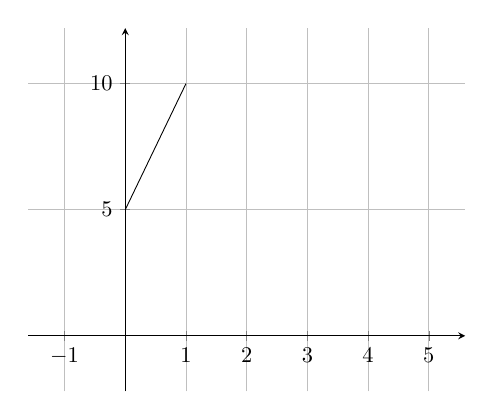
\begin{tikzpicture}[scale=0.81, trim axis right]
            \begin{axis}[grid=both,xmin=-1,xmax=5,ymin=-1,ymax=11,axis lines=middle,enlargelimits]
            \addplot[domain=0:1] {5*x+5};            
            \end{axis}
            
            \end{tikzpicture}

\end{document}
